%
% section 4.1.2
%
\subsection{Πρωτόκολλο UDP -- Δομή Πακέτου}

Το πρωτόκολλο UDP, User Datagram Protocol, βρίσκεται επίσης στο επίπεδο μεταφοράς αλλά είναι ένα αρκετά απλούστερο πρωτόκολλο σε σχέση με το TCP. To UDP χρησιμοποιεί αυτοδύναμα πακέτα για τη μεταφορά των δεδομένων του και είναι πρωτόκολλο χωρίς σύνδεση: η μετάδοση ξεκινά αμέσως χωρίς να υπάρχει από πριν συνεννόηση με την άλλη πλευρά. 

Μερικές ακόμα σημαντικές διαφορές με το TCP είναι:

\begin{itemize}
\item Το UDP δεν μπορεί να τεμαχίσει δεδομένα. Αν επιθυμούμε κάτι τέτοιο θα πρέπει να το αναλάβει το επίπεδο εφαρμογής.
\item Το UDP δεν εξασφαλίζει αξιόπιστη μετάδοση δεδομένων. Τα πακέτα είναι αυτοδύναμα και δεν παρέχεται αναμετάδοση σε περίπτωση απώλειας ή καταστροφής πακέτων. Αν κάτι τέτοιο είναι επιθυμητό, θα πρέπει και πάλι να το αναλάβει το επίπεδο εφαρμογής.
\end{itemize}

Από την άλλη, το UDP είναι αρκετά απλούστερο πρωτόκολλο. Η επικεφαλίδα του είναι μόνο 8 οκτάδες, άρα διαθέτει περισσότερο χώρο για να μεταφέρει χρήσιμα δεδομένα. Καθώς δεν χρειάζεται εγκατάσταση σύνδεσης η μετάδοση μπορεί να ξεκινήσει άμεσα. Η έλλειψη ελέγχων σημαίνει συνήθως μεγαλύτερη ταχύτητα μετάδοσης δεδομένων και δεν χρησιμοποιούνται πόροι του δικτύου για τη μετάδοση πληροφοριών που δεν αποτελούν πραγματικά δεδομένα χρήστη (όπως αναφέρει το σχολικό βιβλίο, λιγότερο overhead, λιγότερη επιβάρυνση δηλ. από δεδομένα ελέγχου κλπ).

\begin{figure}[!ht]
 \centering
 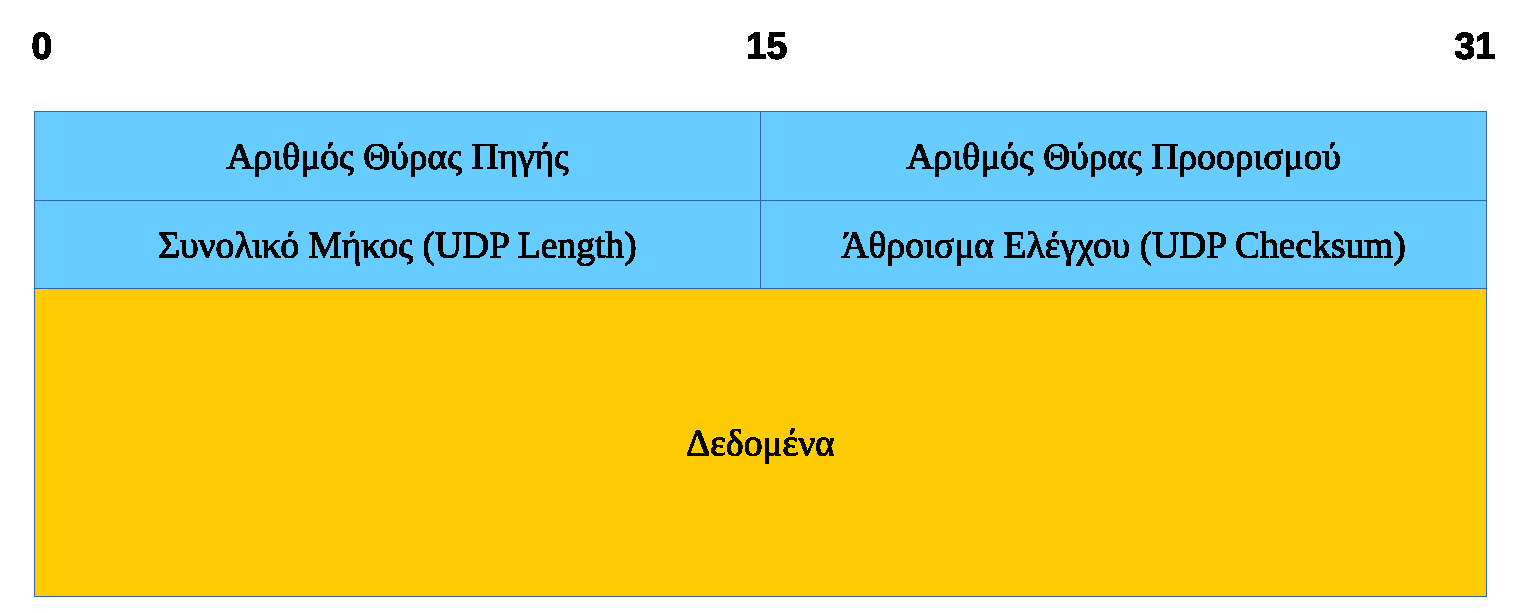
\includegraphics[width=0.95\textwidth]{images/chapter4/4-4}
 \caption {\textsl{Πεδία Επικεφαλίδας UDP Πακέτου}}
 \label{4-4}
\end{figure}

Η επικεφαλίδα του UDP έχει μέγεθος 8 οκτάδων (σχήμα \ref{4-4}) και τα πεδία της είναι:

\begin{itemize}
\item \textbf{Αριθμοί Θύρας Προέλευσης και Προορισμού (Source / Destination Ports:} Με μέγεθος 16 bit το καθένα, εξυπηρετούν τον ίδιο ακριβώς σκοπό με τις θύρες του TCP.
\item \textbf{Μήκος Datagram (Length):} Το ελάχιστο μέγεθος είναι 8 bytes (μόνο η επικεφαλίδα δηλαδή) και το μέγιστο 65535 bytes (64 Kb) μαζί με την επικεφαλίδα. Το πεδίο αυτό έχει (προφανώς) μέγεθος 16 bit.
\item \textbf{Το Άθροισμα Ελέγχου (Checksum):} Προαιρετικό πεδίο μεγέθους 16 bit. Χρησιμεύει για επαλήθευση ορθότητας της επικεφαλίδας και των δεδομένων στον παραλήπτη και λειτουργεί παρόμοια με το αντίστοιχο πεδίο του TCP. 
\end{itemize}

Είναι προφανές ότι το πρωτόκολλο TCP χρησιμοποιείται όπου απαιτείται αξιόπιστη μεταφορά των δεδομένων ενώ το UDP σε εφαρμογές που δεν έχει τόση σημασία η πληρότητα της μεταφοράς των δεδομένων σε σχέση με την ταχύτητα που θα παραληφθούν.

Τέτοιες εφαρμογές είναι:

\begin{itemize}
\item Όσες μεταδίδουν εικόνα, βίντεο και ήχο σε πραγματικό χρόνο (ρόες -- streams -- δεδομένων). Για παράδειγμα εφαρμογές τηλεδιάσκεψης, εφαρμογές τηλεόρασης μέσω Διαδικτύου, τηλεφωνία μέσω IP (VoIP), Internet Radio κλπ. Στις περιπτώσεις αυτές μας ενδιαφέρει τα δεδομένα να φτάνουν στη σωστή χρονική στιγμή ενώ μερικές απώλειες δεν είναι σημαντικές αφού επηρεάζουν μόνο για λίγο την ποιότητα αναπαραγωγής.
\item Εξυπηρετητές (servers) οι οποίοι απαντούν σε μικρά αιτήματα τεράστιου αριθμού από πελάτες όπως π.χ. σε δικτυακά online παιχνίδια. Οι συγκεκριμένοι εξυπηρετητές μπορούν να αντιμετωπίσουν έτσι αρκετά μεγαλύτερο φορτίο εργασίας από ότι αν χρησιμοποιούσαν TCP, καθώς το UDP πρωτόκολλο είναι αρκετά απλούστερο και δεν χρειάζεται να ανταλλάσσουν πληροφορίες ελέγχου και κατάστασης της σύνδεσης. 
\end{itemize}

Όπως αναφέραμε ωστόσο, αν θέλουμε να έχουμε αξιοπιστία, κατατεμαχισμό δεδομένων ή έλεγχο ροής στο UDP, θα πρέπει να μεταφέρουμε αυτές τις ενέργειες στο επίπεδο εφαρμογής. Υπάρχει επίσης το πρόβλημα της δικτυακής συμφόρησης που προκύπτει όταν κάποιος αποστολέας UDP πλημμυρίσει το δίκτυο με πακέτα. Για το σκοπό αυτό οι δρομολογητές πρέπει να χρησιμοποιούν τεχνικές ελέγχουν ώστε να μπορούν να απορρίπτουν ή να αποθηκεύουν προσωρινά πακέτα IP που ενθυλακώνουν UDP πακέτα για να αποφεύγεται η κατάρρευση (Hint: Το πακέτο IP περιέχει πεδίο στην επικεφαλίδα που αναγράφει από ποιο πρωτόκολλο του επιπέδου μεταφοράς προέρχονται τα δεδομένα που μεταφέρει. Το σχολικό βιβλίο εδώ γράφει για άλλη μια φορά ότι οι δρομολογητές απορρίπτουν πακέτα UDP, που είναι, φυσικά, λάθος).